\documentclass[multi=tikzpicture,border=8pt]{standalone}
\usepackage[T1]{fontenc}
\usepackage{lmodern}
\usepackage{amsmath}
\usepackage{xcolor}
\usepackage{tikz}
\usetikzlibrary{arrows.meta,positioning,fit,backgrounds,calc}
\begin{document}

% ---- Diagram 1: end-to-end pipeline ----
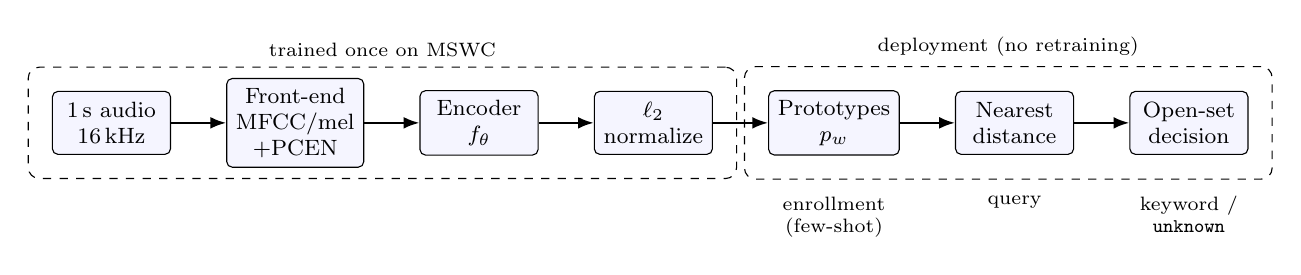
\begin{tikzpicture}[
  node distance=5mm and 7mm,
  box/.style={draw,rounded corners=2pt,align=center,minimum height=8mm,
              minimum width=15mm,font=\footnotesize,fill=blue!4},
  arr/.style={-{Latex[length=2mm]},thick},
  small/.style={font=\scriptsize,align=center}]
\node[box] (wav) {1\,s audio\\16\,kHz};
\node[box,right=of wav] (feat) {Front-end\\MFCC/mel\\$+$PCEN};
\node[box,right=of feat] (enc) {Encoder\\$f_\theta$};
\node[box,right=of enc] (norm) {$\ell_2$\\normalize};
\node[box,right=of norm] (proto) {Prototypes\\$p_w$};
\node[box,right=of proto] (dist) {Nearest\\distance};
\node[box,right=of dist] (dec) {Open-set\\decision};
\draw[arr](wav)--(feat);\draw[arr](feat)--(enc);\draw[arr](enc)--(norm);
\draw[arr](norm)--(proto);\draw[arr](proto)--(dist);\draw[arr](dist)--(dec);
\node[small,below=4mm of proto]{enrollment\\(few-shot)};
\node[small,below=4mm of dist]{query};
\node[small,below=4mm of dec]{keyword /\\\texttt{unknown}};
\begin{scope}[on background layer]
\node[draw,dashed,rounded corners,fit=(wav)(norm),inner sep=3mm,
      label={[font=\scriptsize]above:trained once on MSWC}]{};
\node[draw,dashed,rounded corners,fit=(proto)(dec),inner sep=3mm,
      label={[font=\scriptsize]above:deployment (no retraining)}]{};
\end{scope}
\end{tikzpicture}

% ---- Diagram 2: DSCNN-L ----
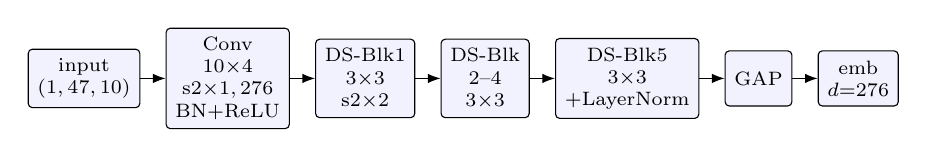
\begin{tikzpicture}[
  font=\scriptsize, node distance=3.2mm,
  b/.style={draw,rounded corners=1.5pt,minimum height=7mm,align=center,fill=blue!5},
  a/.style={-{Latex[length=1.6mm]}}]
\node[b] (in) {input\\$(1,47,10)$};
\node[b,right=of in] (c0) {Conv\\$10{\times}4$\\s$2{\times}1$,\,276\\BN+ReLU};
\node[b,right=of c0] (d1) {DS-Blk1\\$3{\times}3$\\s$2{\times}2$};
\node[b,right=of d1] (d2) {DS-Blk\\2--4\\$3{\times}3$};
\node[b,right=of d2] (d5) {DS-Blk5\\$3{\times}3$\\+LayerNorm};
\node[b,right=of d5] (gap) {GAP};
\node[b,right=of gap] (emb) {emb\\$d{=}276$};
\draw[a](in)--(c0);\draw[a](c0)--(d1);\draw[a](d1)--(d2);\draw[a](d2)--(d5);
\draw[a](d5)--(gap);\draw[a](gap)--(emb);
\end{tikzpicture}

% ---- Diagram 3: EdgeSpot-Full ----
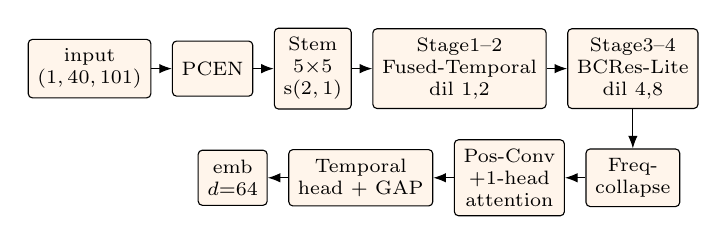
\begin{tikzpicture}[
  font=\scriptsize, node distance=2.6mm,
  b/.style={draw,rounded corners=1.5pt,minimum height=7mm,align=center,fill=orange!8},
  a/.style={-{Latex[length=1.6mm]}}]
\node[b] (in) {input\\$(1,40,101)$};
\node[b,right=of in] (pc) {PCEN};
\node[b,right=of pc] (st) {Stem\\$5{\times}5$\\s$(2,1)$};
\node[b,right=of st] (s12) {Stage1--2\\Fused-Temporal\\dil 1,2};
\node[b,right=of s12] (s34) {Stage3--4\\BCRes-Lite\\dil 4,8};
\node[b,below=5mm of s34] (fc) {Freq-\\collapse};
\node[b,left=of fc] (att) {Pos-Conv\\$+$1-head\\attention};
\node[b,left=of att] (th) {Temporal\\head + GAP};
\node[b,left=of th] (emb) {emb\\$d{=}64$};
\draw[a](in)--(pc);\draw[a](pc)--(st);\draw[a](st)--(s12);\draw[a](s12)--(s34);
\draw[a](s34)--(fc);\draw[a](fc)--(att);\draw[a](att)--(th);\draw[a](th)--(emb);
\end{tikzpicture}

\end{document}
